%%%%%%%%%%%%%%%%%%%%%%%%%%%%%%%%%%%%%%%%%
% NIWeek 2014 Poster by T. Reveyrand
% www.microwave.fr
% http://www.microwave.fr/LaTeX.html
% ---------------------------------------
% 
% Original template created by:
% Brian Amberg (baposter@brian-amberg.de)
%
% This template has been downloaded from:
% http://www.LaTeXTemplates.com
%
% License:
% CC BY-NC-SA 3.0 (http://creativecommons.org/licenses/by-nc-sa/3.0/)
%
%%%%%%%%%%%%%%%%%%%%%%%%%%%%%%%%%%%%%%%%%

%----------------------------------------------------------------------------------------
%	PACKAGES AND OTHER DOCUMENT CONFIGURATIONS
%----------------------------------------------------------------------------------------

\documentclass[a0paper,portrait]{baposter}

\usepackage[font=small,labelfont=bf]{caption} % Required for specifying captions to tables and figures
\usepackage{booktabs} % Horizontal rules in tables
\usepackage{relsize} % Used for making text smaller in some places

\usepackage{amsmath,amsfonts,amssymb,amsthm} % Math packages
\usepackage{eqparbox}

\usepackage{textcomp}
\usepackage{multicol}
\usepackage{wrapfig} % Allows wrapping text around tables and figures

\usepackage{enumerate} % Customized item style
\usepackage{mdwlist} % Tight lists
\usepackage{threeparttable}
\usepackage{tcolorbox}
\usepackage{multirow}
\usepackage{setspace} % For 'spacing' environment
\usepackage{dashrule} % For hdashrule

\renewcommand{\familydefault}{\sfdefault}

\graphicspath{{Fig/}} % Directory in which figures are stored

 \definecolor{bordercol}{RGB}{40,40,40} % Border color of content boxes
 \definecolor{headercol1}{RGB}{186,215,230} % Background color for the header in the content boxes (left side)
 \definecolor{headercol2}{RGB}{120,120,120} % Background color for the header in the content boxes (right side)
 \definecolor{headerfontcol}{RGB}{0,0,0} % Text color for the header text in the content boxes
 \definecolor{boxcolor}{RGB}{210,235,250} % Background color for the content in the content boxes
 
 \definecolor{Mycolor1}{RGB}{160,183,210}
 \definecolor{Mycolor2}{RGB}{177,202,228}
 \definecolor{Mycolor3}{RGB}{255,255,255}
 
 \definecolor{lightgray}{gray}{0.95}



% Define a new command for text subscript
\newcommand{\tsub}{\textsubscript}
\newcommand{\tup}{\textsuperscript}

 \newcommand{\compresslist}{%
 \setlength{\itemsep}{0pt}%
 \setlength{\parskip}{0pt}%
 \setlength{\parsep}{0pt}%
 }
 
\usepackage{enumitem}
\setlist[itemize]{noitemsep, topsep=0pt, leftmargin=1em}

\renewcommand\labelitemi{$\ast$}

\begin{document}

\begin{poster}{
grid=false,
borderColor=Mycolor1, % Border color of content boxes
headerColorOne=Mycolor2, % Background color for the header in the content boxes (left side)
headerColorTwo=Mycolor3, % Background color for the header in the content boxes (right side)
headerFontColor=headerfontcol, % Text color for the header text in the content boxes
%boxColorOne=boxcolor, % Background color for the content in the content boxes
headershape=roundedright, % Specify the rounded corner in the content box headers
headerfont=\Large\sf\bf, % Font modifiers for the text in the content box headers
textborder=faded,
background=none,
headerborder=open, % Change to closed for a line under the content box headers
boxshade=plain,
colspacing=0.6em,
headerheight=0.12\textheight
}
{
\includegraphics[height=28mm]{rsph2.png}}
%
%----------------------------------------------------------------------------------------
%	TITLE AND AUTHOR NAME
%----------------------------------------------------------------------------------------
%
{ \bf  \Large {Contribution of Low-Cost Sensor Measurements to the Prediction of PM\tsub{2.5} Levels: A Case Study in Imperial County, California, USA} }
%\Large \it A} % Poster title
{\vspace{0.3em} \smaller Jianzhao Bi$^1$, Jennifer Stowell$^1$, Edmund Seto$^2$, Paul English$^3$, Mohammad Al-Hamdan$^4$, Frank Freedman$^5$, Yang Liu$^{1,\ast}$\\  % Author names
\footnotesize $^1$\it {Department of Environmental Health, Emory University, Atlanta, GA, United States} \\
\footnotesize $^2$\it {Department of Environmental \& Occupational Health Sciences, University of Washington, Seattle, WA, United States} \\
\footnotesize $^3$\it {California Department of Public Health, Richmond, CA, United States} \\
\footnotesize $^4$\it {Universities Space Research Association, NASA Marshall Space Flight Center, Huntsville, AL, United States} \\
\footnotesize $^5$\it {Department of Meteorology and Climate Science, San Jose State University, San Jose, CA, United States}
}
{
\includegraphics[height=30mm]{ises2.png}} 

%----------------------------------------------------------------------------------------
%	Background
%----------------------------------------------------------------------------------------
\headerbox{Background}{name=background,column=0,row=0,span=3}{
Fine particulate matter with aerodynamic diameter less than or equal to 2.5 micrometers (PM\tsub{2.5}) has been contributing to a growing disease burden worldwide. Traditionally, ambient PM\tsub{2.5} exposure assessments have mainly relied on measurements from regulatory monitoring stations. However, as regulatory monitoring is designed to support compliance with ambient air quality standards, it lacks spatial coverage to reflect detailed PM\tsub{2.5} variations at the community level. Recently emerged low-cost PM\tsub{2.5} monitors have the potential to fill in the gaps of regulatory monitoring. With the features of lower instrument cost, ease of use, and portability, low-cost PM\tsub{2.5} monitors can be densely deployed by researchers, grass-roots organizations, and citizen scientists. To date, very few studies, if any, focused on using low-cost sensor measurements to improve high-resolution PM\tsub{2.5} prediction. This study aimed to evaluate the contribution of low-cost measurements to the estimation of PM\tsub{2.5} levels in the regions where sparse regulatory stations alone cannot support reliable predictions.
}

%----------------------------------------------------------------------------------------
%	Data and Methods
%----------------------------------------------------------------------------------------
\headerbox{Data and Methods}{name=data,column=0,row=1,below=background}
{
\includegraphics[width=\textwidth]{domain.png}
\small{\textbf{Fig 1.} Imperial County with AQS (\textcolor{red}{red}) and IVAN (\textcolor{blue}{blue}) sites. Imperial County is in the Southern California border region contiguous to the Mexican state of Baja California. The region has high PM\tsub{2.5} pollution, severe pollution-related health issues, and increased public concerns about the pollution.}

\vspace*{-\baselineskip}
 
\paragraph{AQS} U.S. Environmental Protection Agency Air Quality System, a nationwide regulatory air quality monitoring network. There were 6 AQS stations within the study domain. 

\vspace*{-\baselineskip}

\paragraph{IVAN} Identifying Violations Affecting Neighborhoods, a community-engaged low-cost air quality network in Imperial County. There were 39 calibrated IVAN sites within the study domain. 

\vspace*{-0.3\baselineskip}
\hdashrule{\textwidth}{0.1pt}{0.6mm 0.6mm}
\vspace*{-2\baselineskip}

\paragraph{Prediction Models} Two models with different types of dependent variables were built based on the Random Forest (RF) algorithm. The models shared the same set of independent variables (Table 1).
\begin{itemize}
    \item \textbf{\emph{The AQS-Only Model}}: AQS as the dependent var.
    \item \textbf{\emph{The AQS/IVAN Model}}: merged AQS and IVAN
\end{itemize}

\vspace*{-\baselineskip}

\paragraph{Variable Importance} The RF-specific ``permutation accuracy importance'' used to reflect the relative importance of independent variables in a prediction model. 

\begin{tcolorbox}[boxsep=0pt,left=3pt,right=3pt]
\centering\textbf{The Random-Forest (RF) Prediction Model}
\linespread{0.4}\selectfont
\begin{align*}
    \mathrm{PM}&\mathrm{_{2.5\mathit{st}}=f(\operatorname{Gap-filled}\;AOD_{\mathit{st}}, Auxiliary_{\mathit{st}}},\\
    &\mathrm{Meteorological_{\mathit{st}},\operatorname{Land-use}_\mathit{s},Month_\mathit{t}, Day_\mathit{t})}
\end{align*}
\end{tcolorbox}

\vspace*{-\baselineskip}

\begin{center}
    \textbf{Table 1.} Data sources\\
{\renewcommand{\arraystretch}{0.7}%
\begin{threeparttable}
\footnotesize
\begingroup\setlength{\fboxsep}{0pt}
\colorbox{lightgray}{%
\begin{tabular}{cccc}
\toprule
\textbf{Type}              & \textbf{Source} & \textbf{Time Freq.} & \textbf{Spatial Res.} \\ \midrule
\multirow{2}{*}{PM}     & AQS             & Daily               & --                    \\
                           & IVAN            & Hourly              & --                    \\ \midrule
AOD                        & MAIAC           & Daily               & 1-km                  \\ \midrule
Met.                       & HRRR            & Hourly              & 3-km                  \\ \midrule
Land-use                   & Multiple        & Invariant           & $\leq$1-km        \\ \midrule
\multirow{2}{*}{Auxiliary} & Conv. Layer     & Daily               & 1-km                  \\
                           & PM\tsub{2.5}/PM\tsub{10}      & Daily               & 1-km                  \\ \bottomrule
\end{tabular}
}\endgroup
\end{threeparttable}
}
\end{center}

}

%----------------------------------------------------------------------------------------
%	Implications
%----------------------------------------------------------------------------------------
\headerbox{Implications}{name=implications,column=1,row=1,span=2,below=background}
{

\begin{itemize}
    \item The combination of dense and frequent low-cost measurements, spatiotemporally continuous satellite AOD retrievals, and accurate regulatory measurements is a possible solution for the regions with sparse regulatory stations to derive PM\tsub{2.5} distribution details
    \item Introducing low-cost sensor data can significantly change the predicted PM\tsub{2.5} distribution, which appears to provide additional information regarding the pollution
    \item Low-cost sensor data bring noise into model predictions, and formal treatment of measurement errors is necessary for quantitative characterization of PM\tsub{2.5}
\end{itemize}

}

%----------------------------------------------------------------------------------------
%	Predictions of PM2.5
%----------------------------------------------------------------------------------------
\headerbox{PM\tsub{2.5} Modeling Results}{name=modeling,column=1,row=1,span=2,below=implications}
{
\begin{center}
    \textbf{Table 2.} Cross-validation performance of the models\\
    \begin{threeparttable}
    \begingroup\setlength{\fboxsep}{0pt}
    \colorbox{lightgray}{%
    \begin{tabular}{cccccc}
    \toprule
    \textbf{Dependent Var.}     & \textbf{N}      & \textbf{Overall CV R\tup{2}} & \textbf{Spatial CV R\tup{2}} & \textbf{Temporal CV R\tup{2}} & \textbf{CV RMSPE} \\
    \midrule
    AQS-Only  & 1,617  & 0.53          & 0.24          & 0.55           & 3.76 $\mathrm{\mu g/m^3}$ \\
    AQS/IVAN  & 12,902 & 0.73          & 0.63          & 0.70           & 3.72 $\mathrm{\mu g/m^3}$\\
    \bottomrule
    \end{tabular}
    }\endgroup
    \end{threeparttable}
\end{center}

\vspace*{-0.8\baselineskip}

\begin{itemize}
    \item The AQS measurements within the domain could not support reliable PM\tsub{2.5} predictions, and the IVAN measurements, albeit noisier, served as an effective supplement to improve modeling performance and prediction quality 
    \begin{itemize}
        \item The overall CV R\tup{2} of the AQS-only model was low and the spatial CV R\tup{2} was even lower (Table 2)
        \item Since all AQS stations were close to the major roads, the AQS-only model overemphasized the near-road pollution which was believed to be unrealistic (Fig. 2)
        \item The addition of IVAN measurements improved overall, spatial, and temporal predictability and contributed to a more natural and realistic PM\tsub{2.5} distribution (Fig. 2)
        \item Elevated importance of source-related land-use parameters indicated that spatially denser IVAN measurements resolved more spatial information of PM\tsub{2.5} (Table 3)
    \end{itemize}
\end{itemize}

\begin{minipage}{0.67\textwidth}
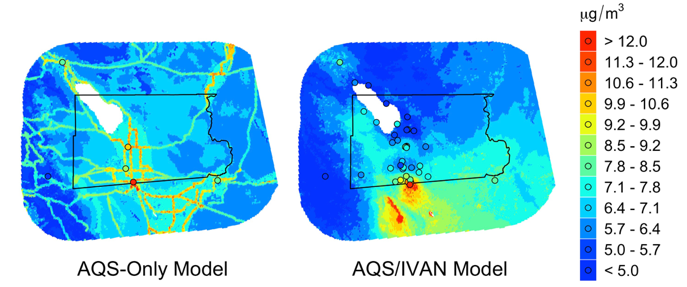
\includegraphics[width=\textwidth]{dist.png}
\textbf{Fig 2.} The mean PM\tsub{2.5} distributions during the study period with the averages of PM\tsub{2.5} levels at the ground stations (points).
\end{minipage}
\begin{minipage}{0.31\textwidth}
{\renewcommand{\arraystretch}{1.1}%
\begin{threeparttable}
\footnotesize
\begingroup\setlength{\fboxsep}{0pt}
\colorbox{lightgray}{%
\begin{tabular}{cc}
\toprule
\textbf{AQS-Only}       & \textbf{AQS/IVAN}        \\
\midrule
Conv. Layer    & Conv. Layer     \\
HPBL           & \textbf{Population}      \\
NDVI           & \textbf{Elevation}       \\
Soil Moist.    & HPBL            \\
Wind Direction & NDVI            \\
Humidity       & \textbf{\% of Grassland} \\
Wind Speed     & PM\tsub{2.5}/PM\tsub{10}      \\
SHFLX          & Soil Moist.     \\
PM\tsub{2.5}/PM\tsub{10}     & \textbf{Dist. to Road}   \\
Ustar          & Temp.            \\
\bottomrule
\end{tabular}
}\endgroup
\end{threeparttable}
\textbf{Table 3.} Top-10 important variables of the models
}
\end{minipage}

\vspace{0.5\baselineskip}

\begin{itemize}
    \item Although AQS was spatially sparser and temporally less-frequent, these ``gold-standard'' measurements were still indispensable in PM\tsub{2.5} prediction
    \begin{itemize}
        \item The model based solely on IVAN had low predictability on AQS measurements with an R\tup{2} of 0.43
        \item The AQS/IVAN model-derived predictions around AQS stations showed more reasonable patterns
    \end{itemize}
\end{itemize}

}


%----------------------------------------------------------------------------------------
%	IVAN Uncertainty
%----------------------------------------------------------------------------------------
\headerbox{Uncertainty of IVAN Measurements}{name=uncertainty,span=2,column=1,row=1, below=modeling}{

\begin{minipage}{0.3\textwidth}
\begin{center}
    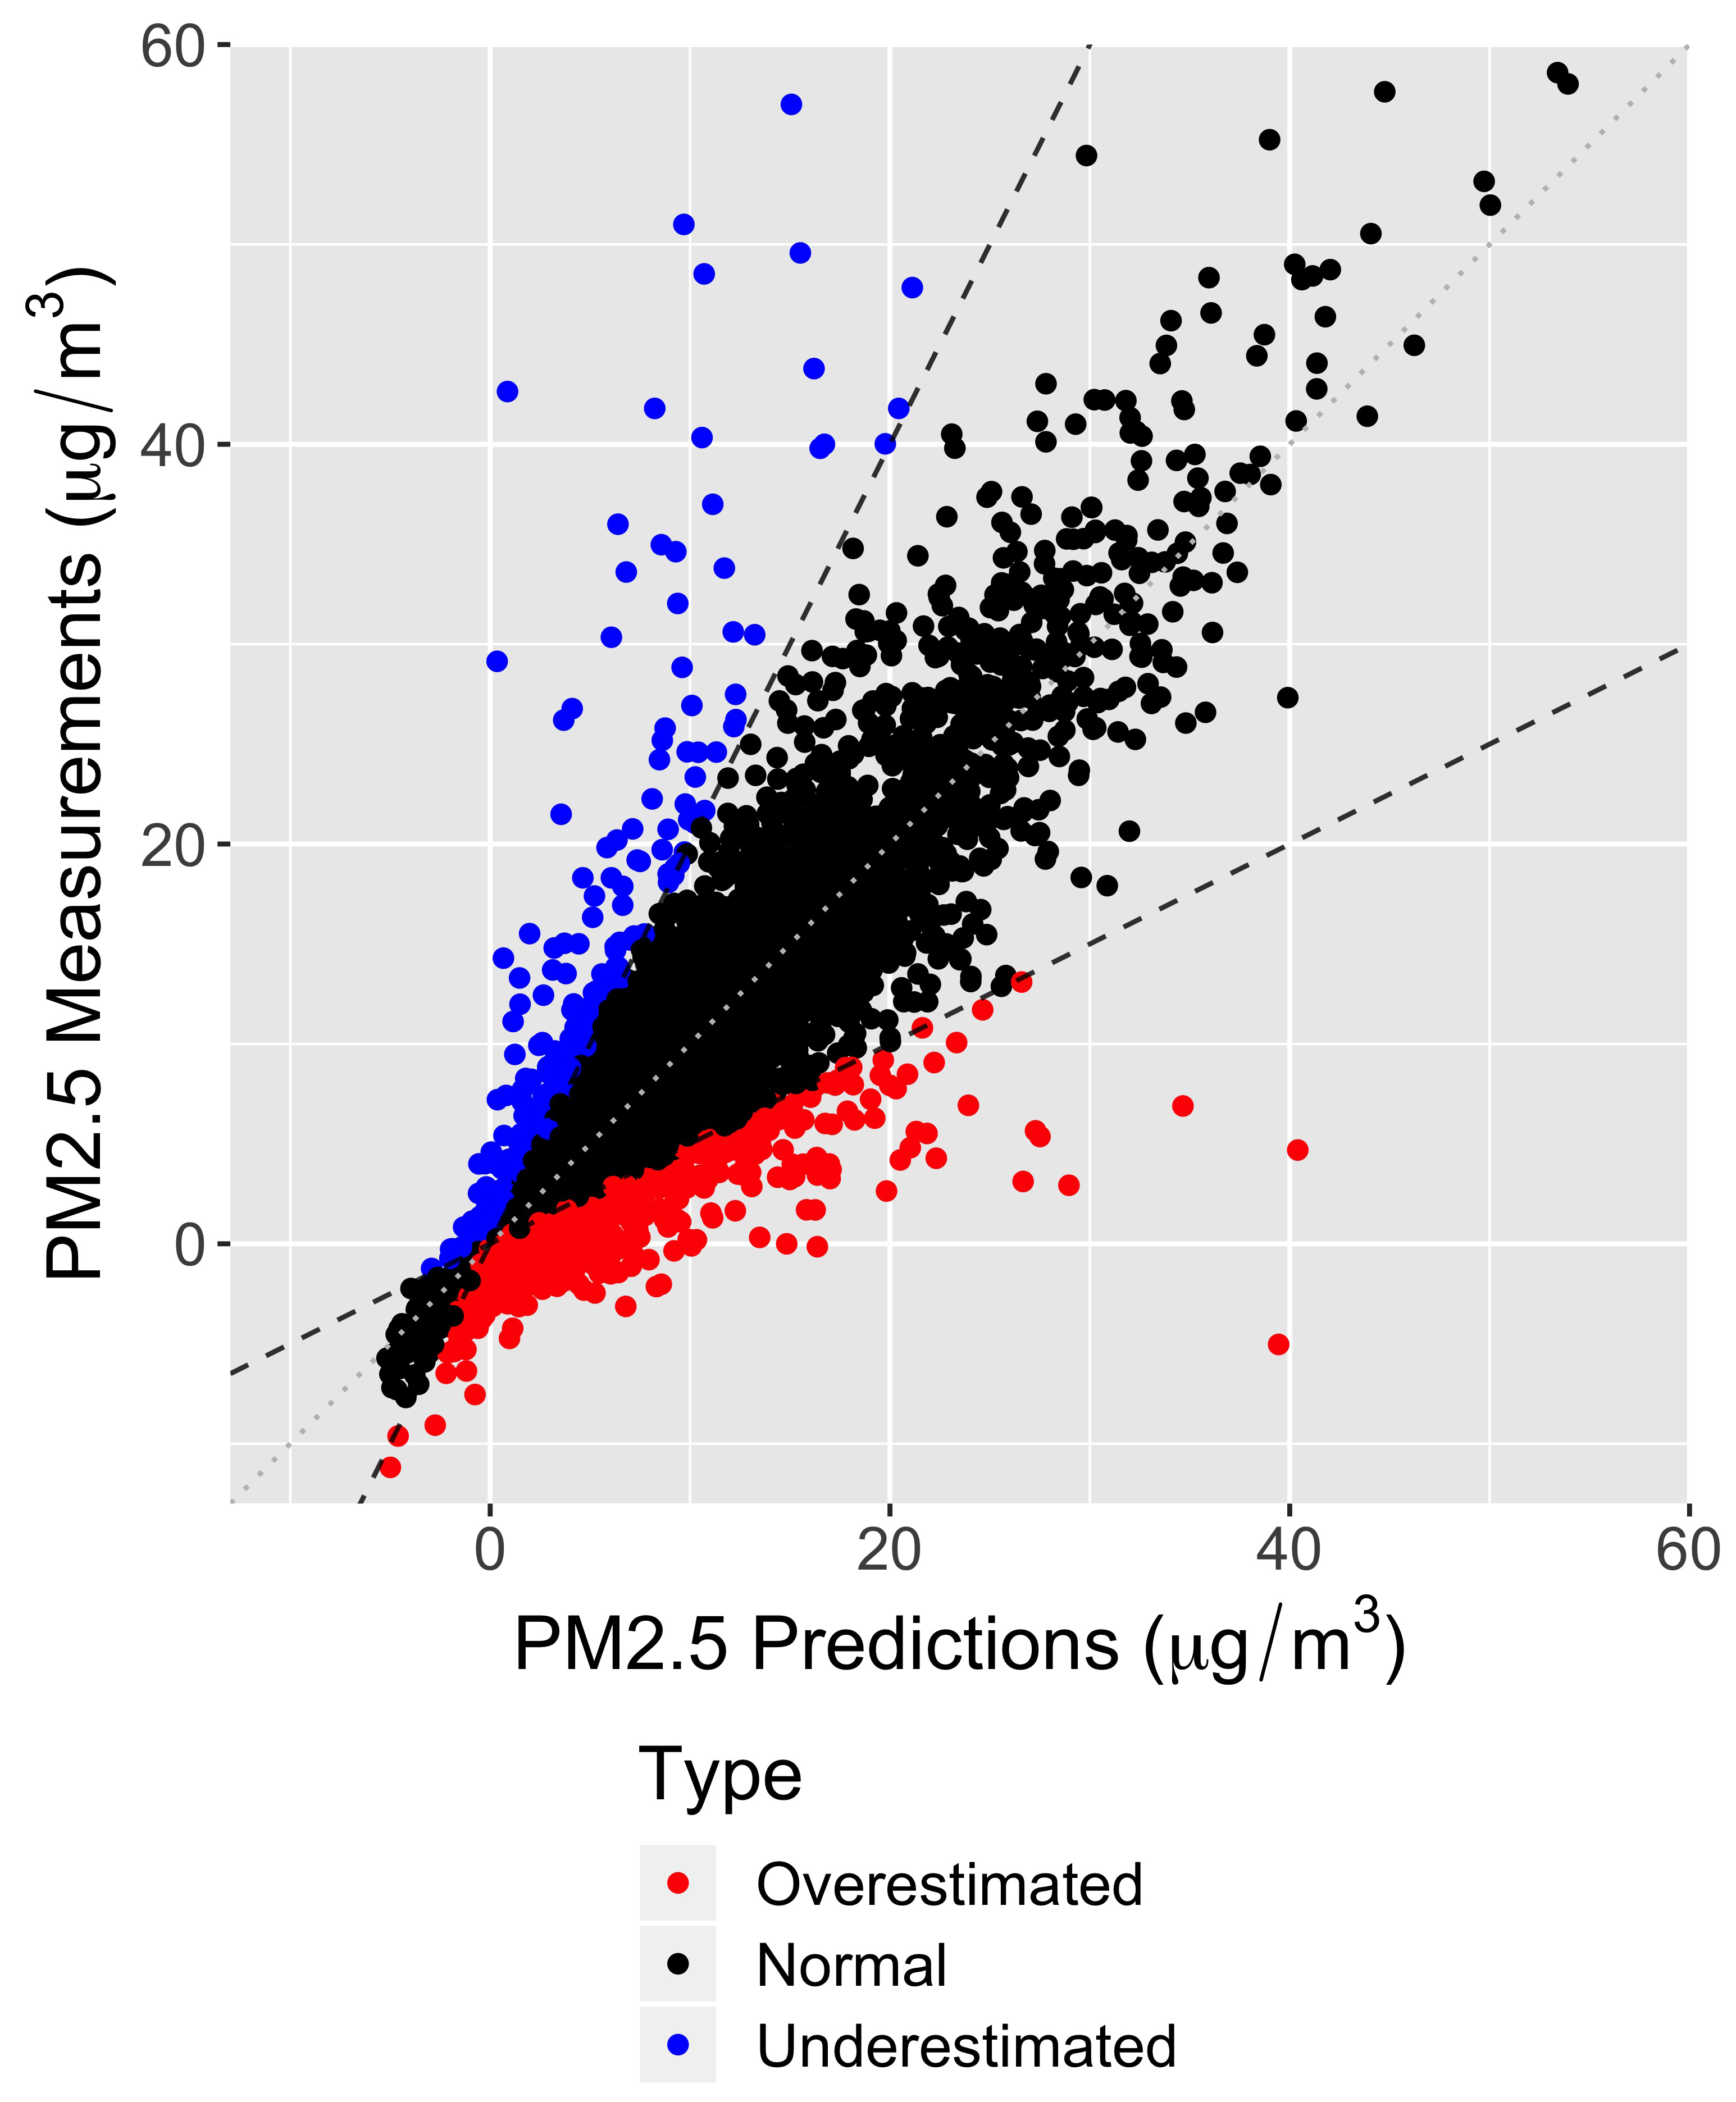
\includegraphics[width=0.95\textwidth]{uncertainty.png}
    \textbf{Fig 3.} IVAN uncertainty
\end{center}
\end{minipage}
\begin{minipage}{0.68\textwidth}
\begin{itemize}
    \item To date, the proposed calibration methods for low-cost sensor measurements mainly focused on correcting systematic biases without reducing random errors commonly existing in the measurements
    \item The residual errors in the low-cost sensor measurements still had considerable impacts on the quality of PM\tsub{2.5} prediction
    \begin{itemize}
        \item The influence of IVAN uncertainty was reflected by substantial outliers in the cross-validation scatter plot, \textit{i.e.}, the red and blue points significantly deviated from the 1:1 line (Fig 3)
        \item As the IVAN uncertainty had a homogeneous effect on the predictions without specific spatiotemporal patterns, it was difficult to pinpoint and remove the inaccurate measurements
    \end{itemize}
    \item Insufficient collocated regulatory/low-cost monitors hindered deeper analyses regarding the uncertainty, and a spatially more extensive low-cost monitoring network should help resolving this issue
\end{itemize}
\end{minipage}

}

%----------------------------------------------------------------------------------------
%	REFERENCES
%----------------------------------------------------------------------------------------
%\headerbox{References}{name=references,column=1,below=conclusion,span=2}{

%}
%----------------------------------------------------------------------------------------
%	ACKNOWLEDGEMENTS
%----------------------------------------------------------------------------------------
\headerbox{Acknowledgements}{name=acknowledgements,column=0,row=2,below=data, above=bottom}{
\begin{spacing}{0.85}
\footnotesize{The work of J. Bi and Y. Liu$^{\ast}$(yang.liu@emory.edu) was supported by NASA Applied Sciences Program (Grant \# NNX16AQ28Q, 80NSSC19K0191, and NNX16AQ91G) and NIEHS (Grant \# R01ES022722). The authors acknowledge the IVAN team of researchers and stakeholders at Comite Civico Del Valle, Inc. lead by Luis Olmedo, Tracking California, and the University of Washington for providing and assisting us in utilizing the IVAN data for this study. 
}
\end{spacing}

} 
\end{poster}
\end{document}
